\subsection{ELISE Projektbeschreibung} \label{elise-subsec}



Elise ist ein Verbundprojekt, welches die Entwicklung eines interaktives und emotionssentives Lernsystem zur Kompetenzentwicklung im Bereich der Gesch{\"a}ftsprozessmanagement plant. 
Hierf{\"u}r kamen f{\"u}nf Partner des Forschungskollegs (FoKoS) der Universit{\"a}t Siegen zusammen – der Lehrstuhl f{\"u}r Wirtschaftsinformatik \& Center for Responsible Innovation \& Design, die Forschungsgruppe Research Group for Patern Recognition, das Institut f{\"u}r Mikrosystemtechnik der Universit{\"a}t Siegen, die Spieleentwickler Limbic Entertainment GmbH und die Softwarehersteller Software AG. 
Zusammen befassen sie sich mit einem interaktiven und emotionssensitiven Lernsystems, im Form eines Spiels, das in einer virtuellen Umgebung erfolgt. 
Zudem befasst sich das Projekt mit der Auswirkung von solcher Systeme hinsichtlich ethischer und gesellschaftlicher Aspekte auf die Akzeptanz potenzieller Nutzerinnen und Nutzer. 
Abbildung \ref{fig-elise} zeigt das vorhaben, welches durch das Projekt Elise verwirklicht werden soll.


\begin{figure}[H] \centering
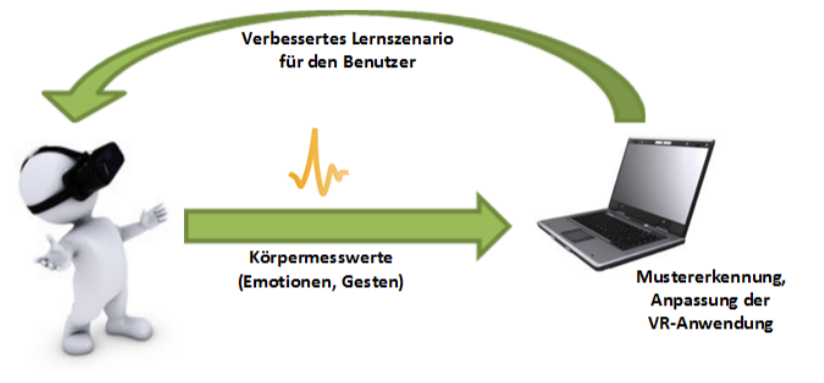
\includegraphics[width=12cm]{Images/elise_projektbeschreibung.png} 
\vspace{-0.3cm} 
\caption{Grobe {\"u}bersicht des Gesamtprojekts\cite{msckroenert}.}
\label{fig-elise} 
\end{figure}